\section{User Interface}\label{sec:ui}

The interface is a single HTML page with a style sheet and about 400 lines of client-side JavaScript
(\file{static/}); there is no framework and no server-side rendering. The page talks only to its own
peer daemon: it posts actions with \code{fetch} and polls \code{/api/messages}, \code{/api/peers},
\code{/api/status}, \code{/api/transfers} and \code{/api/files} every \SI{1.5}{s}. All text received
from the network is inserted with \code{textContent}, never as HTML, so a message cannot inject markup
or scripts into the page.

\fig[fig:ui-chat]{ui_chat_general.png}{Channel view of alice: messages, the peers on the tracker with
their address and ports, connection state, an unread counter for a direct message from bob, and a
notification}{\textwidth}

\Cref{fig:ui-chat} shows the main view. The left column lists the channels and the peers known to the
tracker, each with its user, TCP address and UDP port, and a button that turns dark once the
\code{CONNECT} handshake has succeeded. Clicking a peer opens the direct conversation with it
(\cref{fig:ui-dm}). New messages in a conversation that is not open raise a red counter, a short
notification in the corner, and a counter in the tab title. The footer shows whether the tracker is
reachable.

\begin{figure}[htbp]\centering
\begin{subfigure}{0.49\textwidth}\centering
  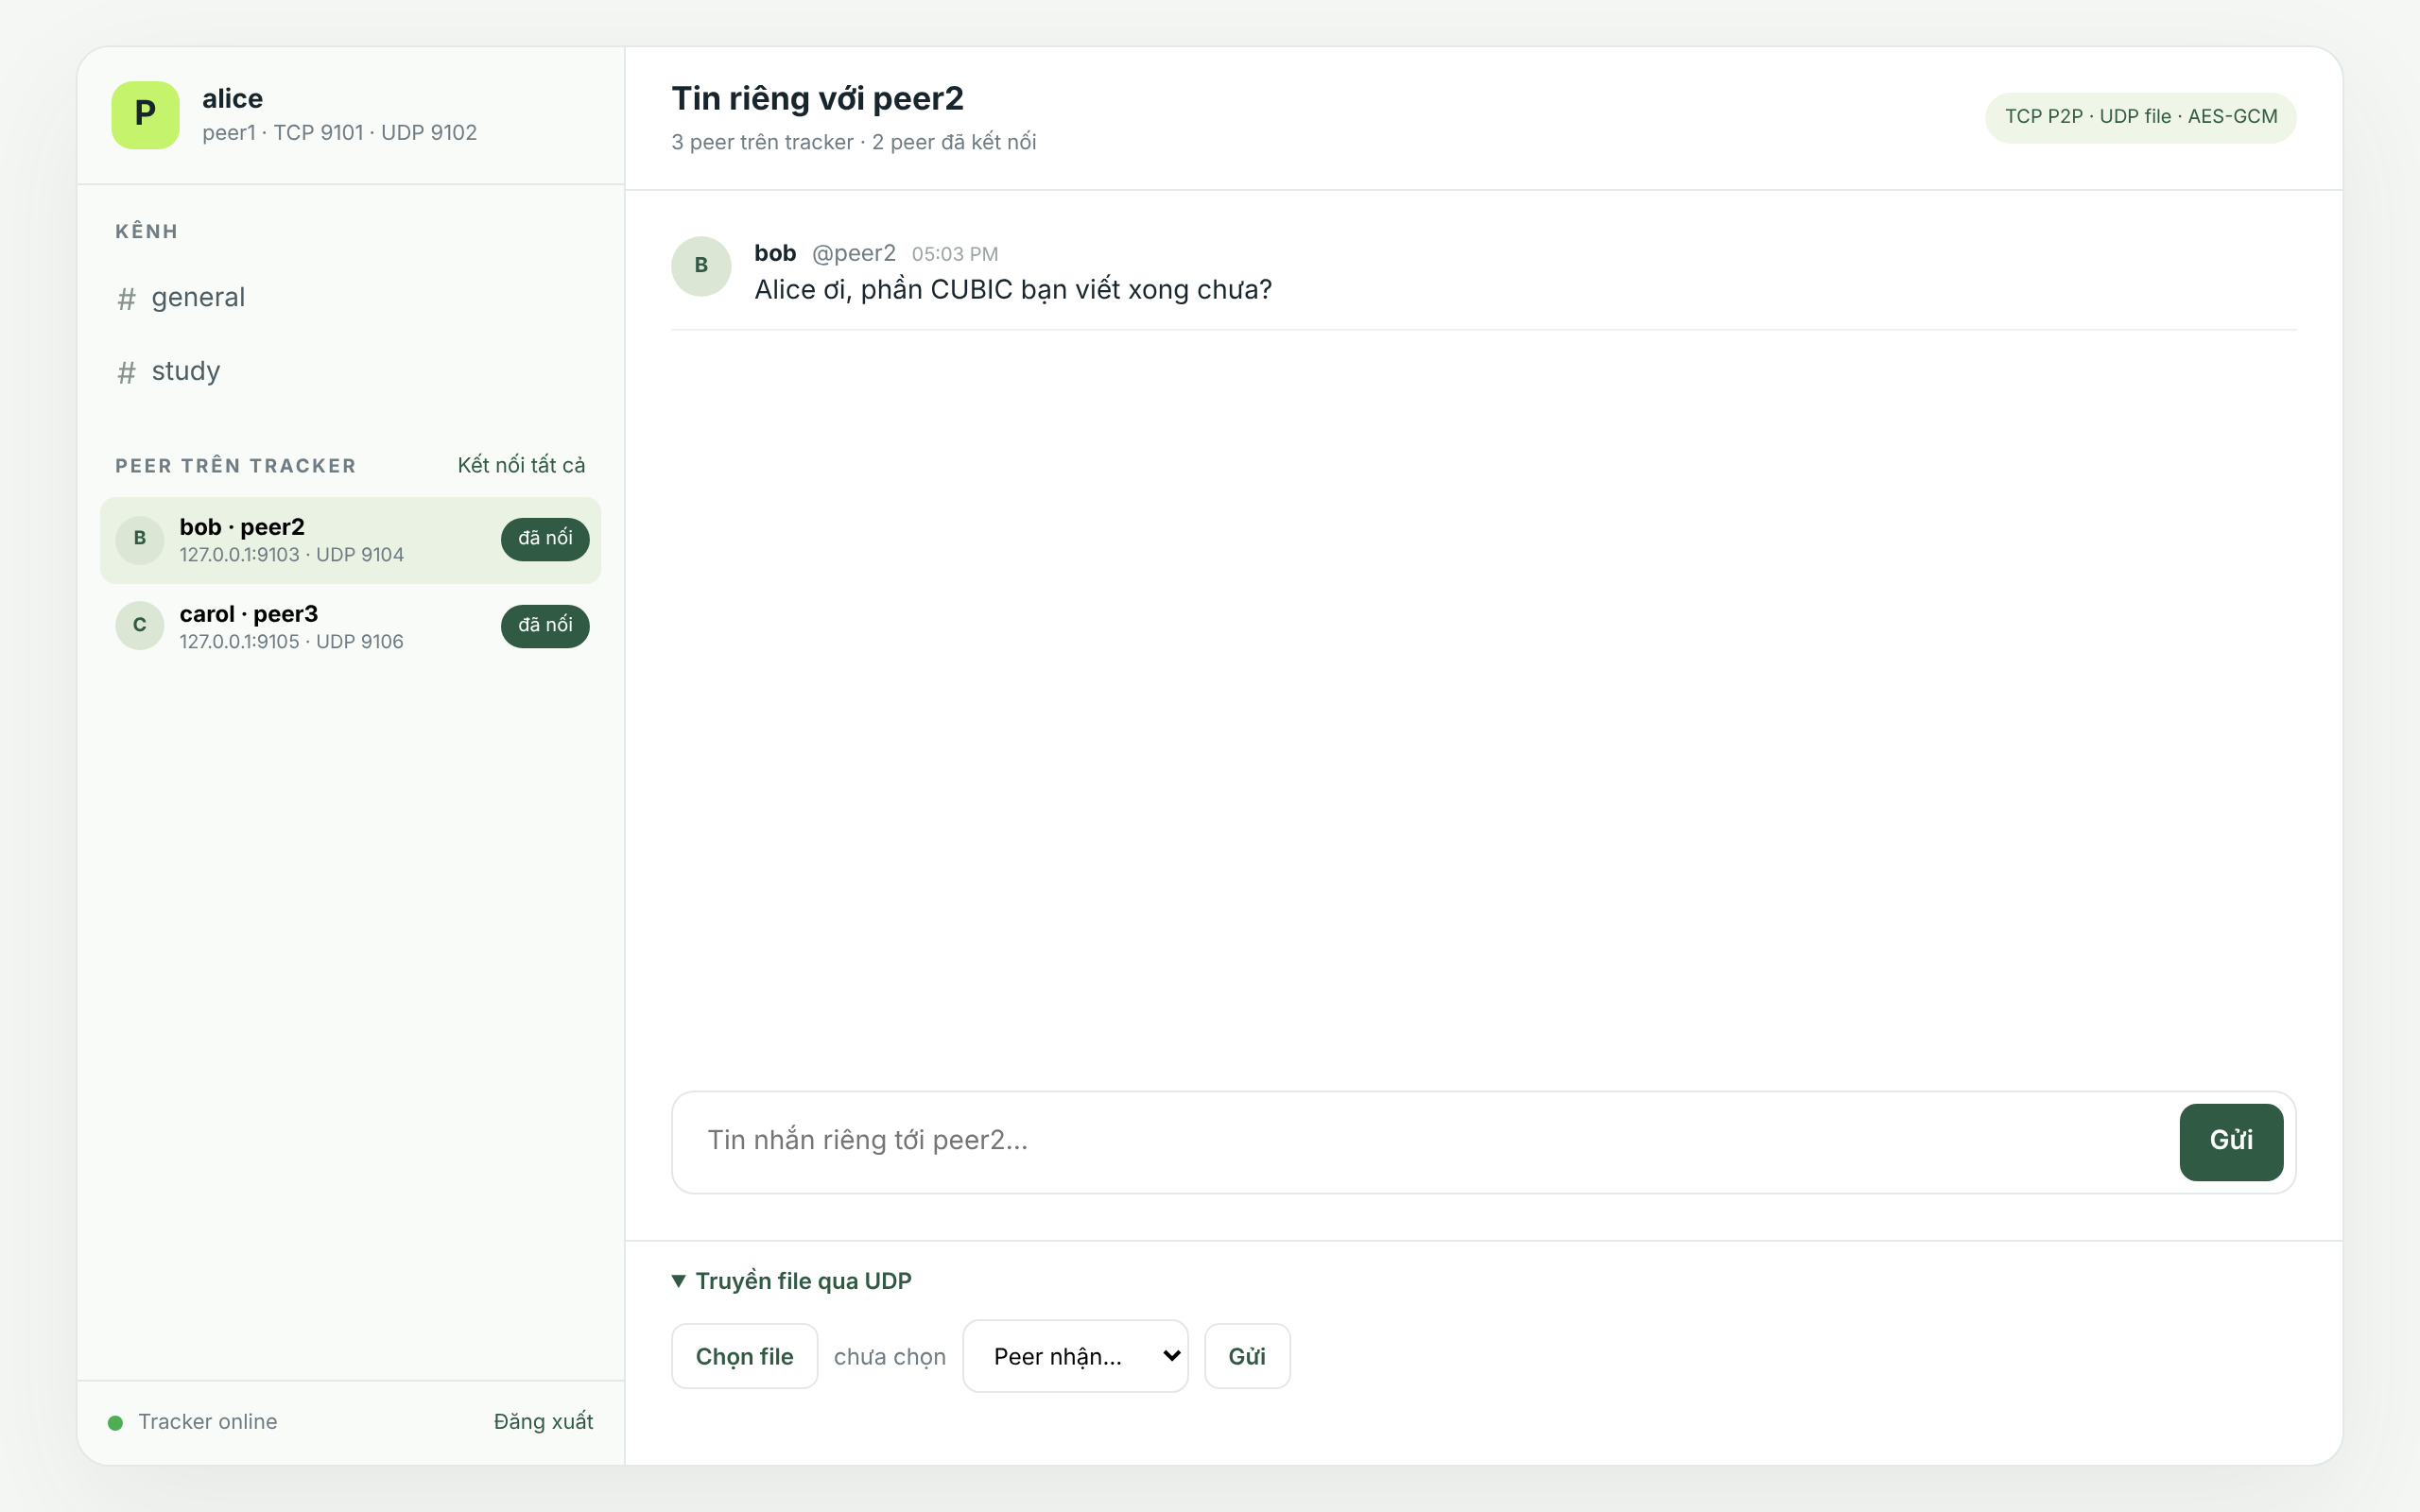
\includegraphics[width=\linewidth]{figures/ui_dm.png}\caption{Direct conversation}\label{fig:ui-dm}
\end{subfigure}\hfill
\begin{subfigure}{0.49\textwidth}\centering
  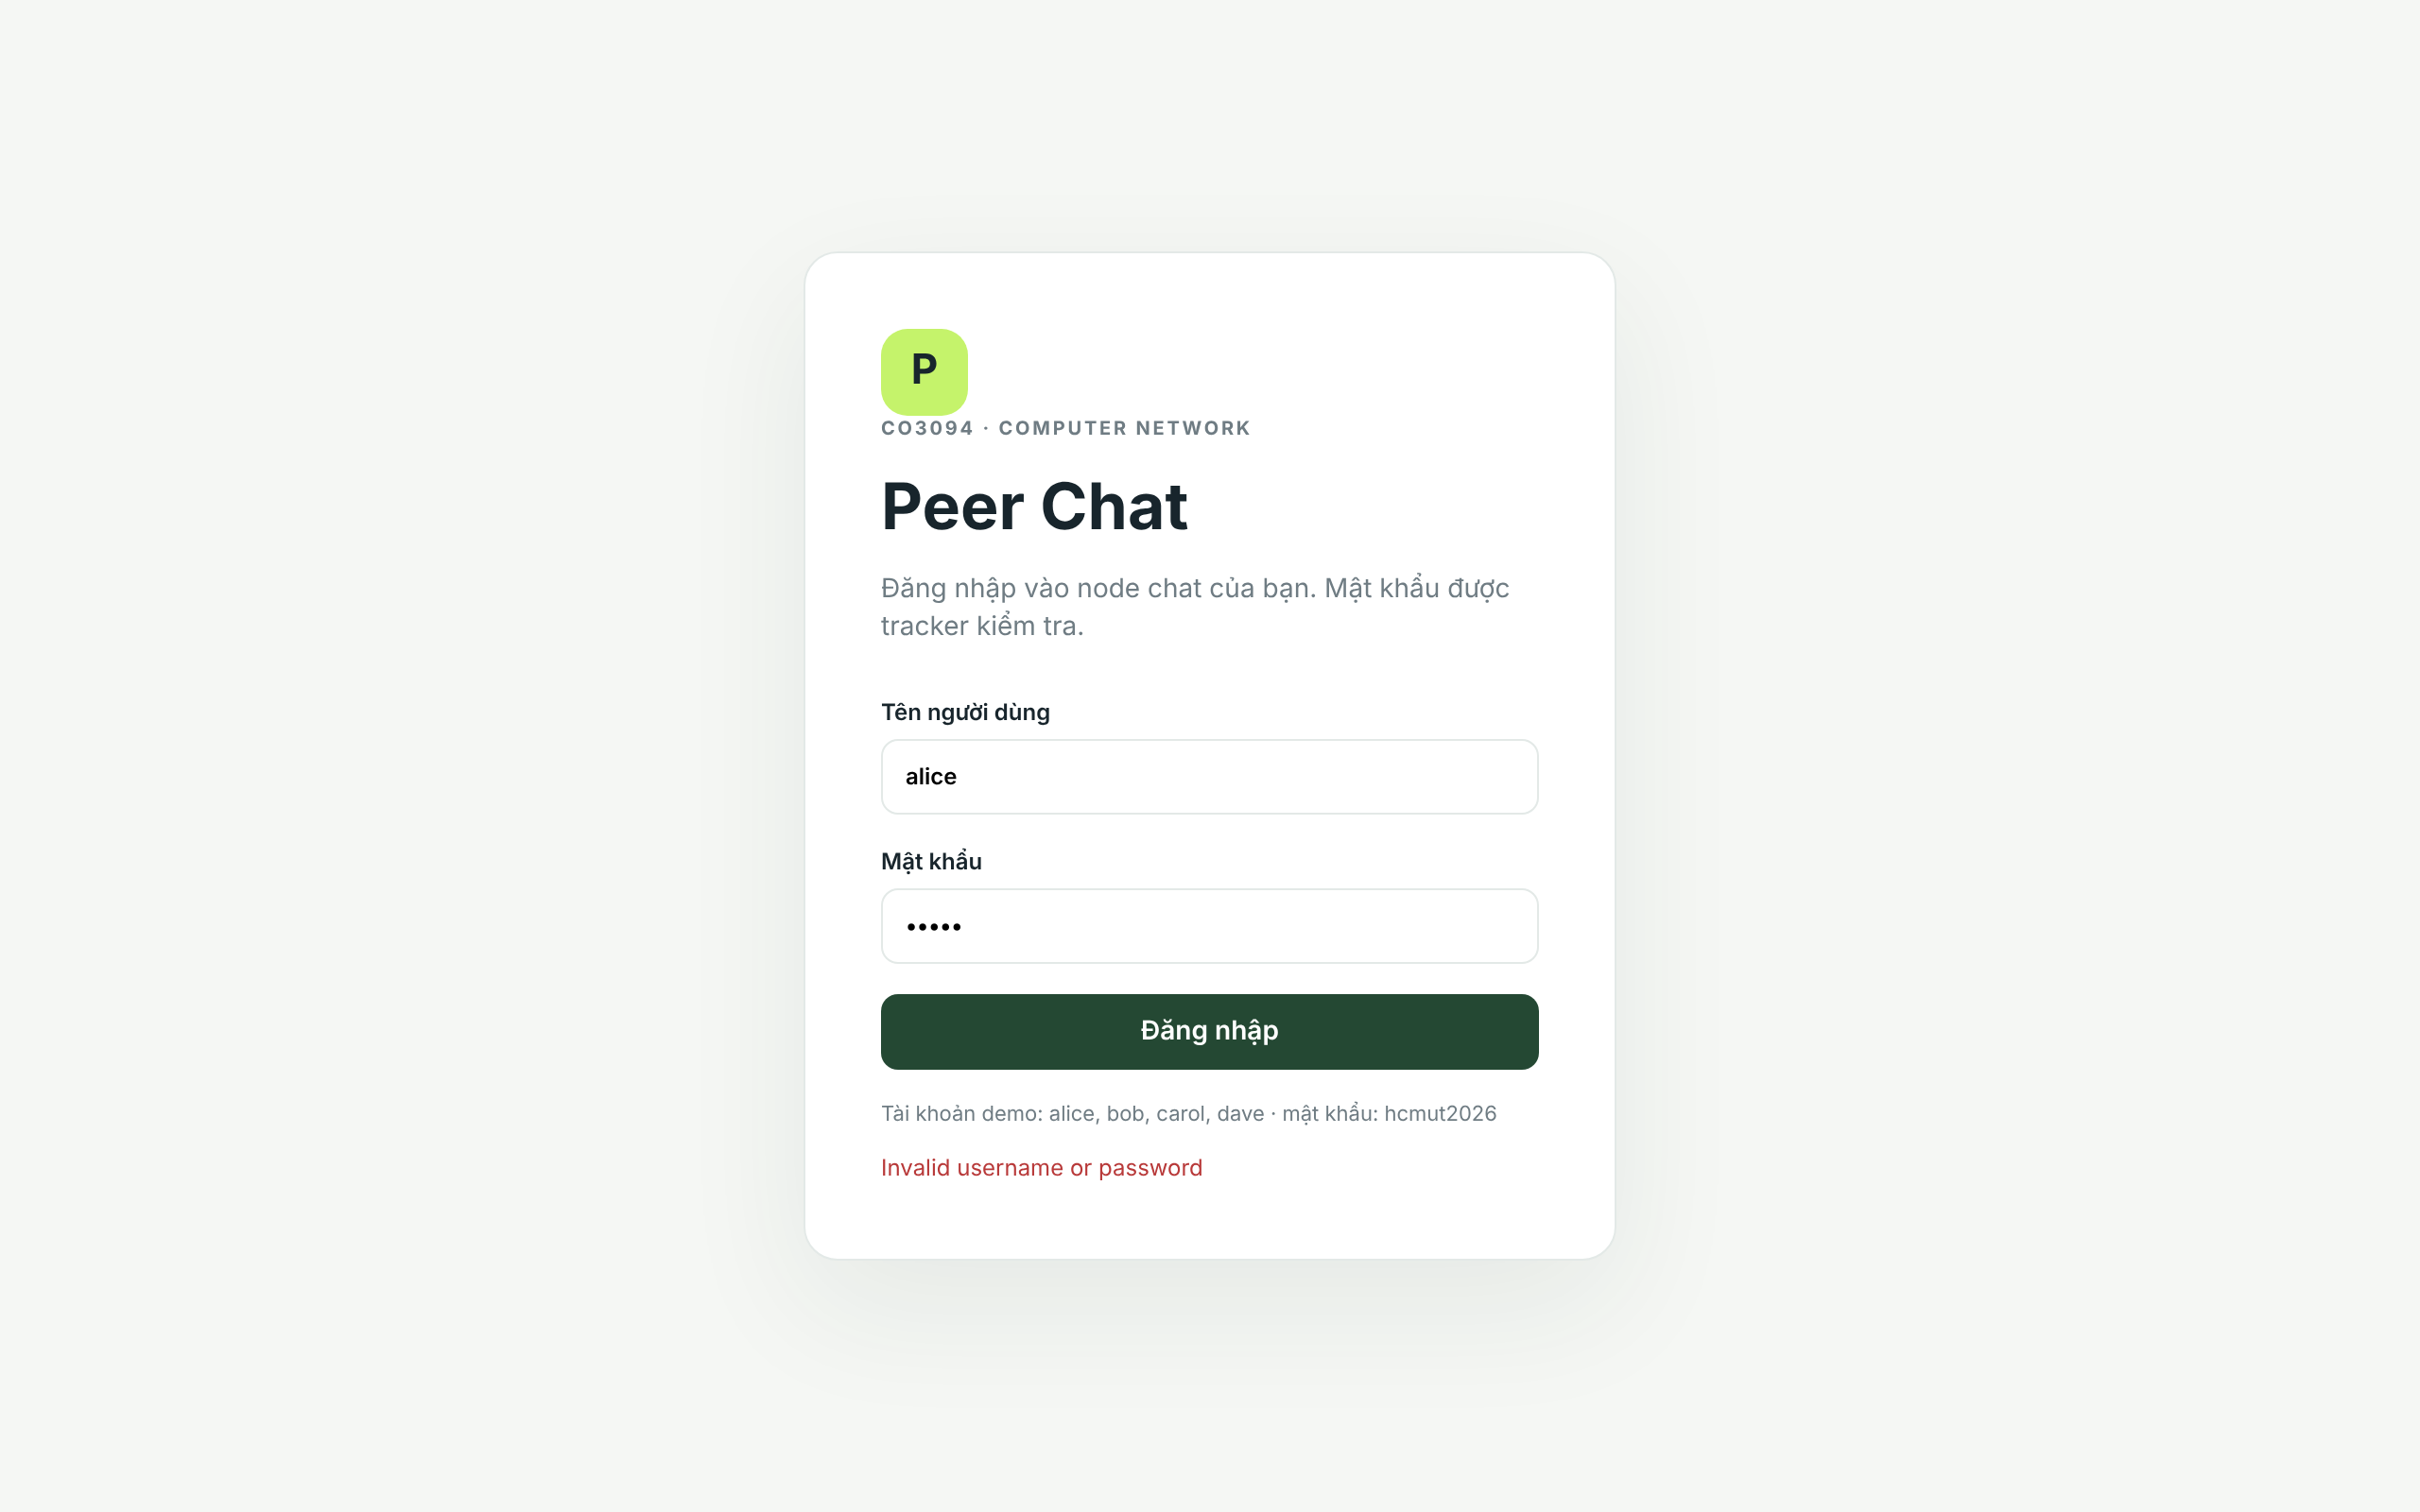
\includegraphics[width=\linewidth]{figures/ui_login_error.png}\caption{Login rejected by the tracker}\label{fig:ui-login}
\end{subfigure}
\caption{Direct messages and login}
\end{figure}

The file panel (\cref{fig:ui-files}) uploads the chosen file to the daemon --- an
\code{XMLHttpRequest} is used because it reports upload progress --- and then shows the UDP transfer
itself: the bar counts acknowledged chunks, and the line below gives the percentage, the size, the
current congestion window and the number of retransmissions, and the throughput when the transfer is
done. The receiver sees an incoming bar and, when the SHA-256 check has passed, a download link.

\begin{figure}[htbp]\centering
\begin{subfigure}{\textwidth}\centering
  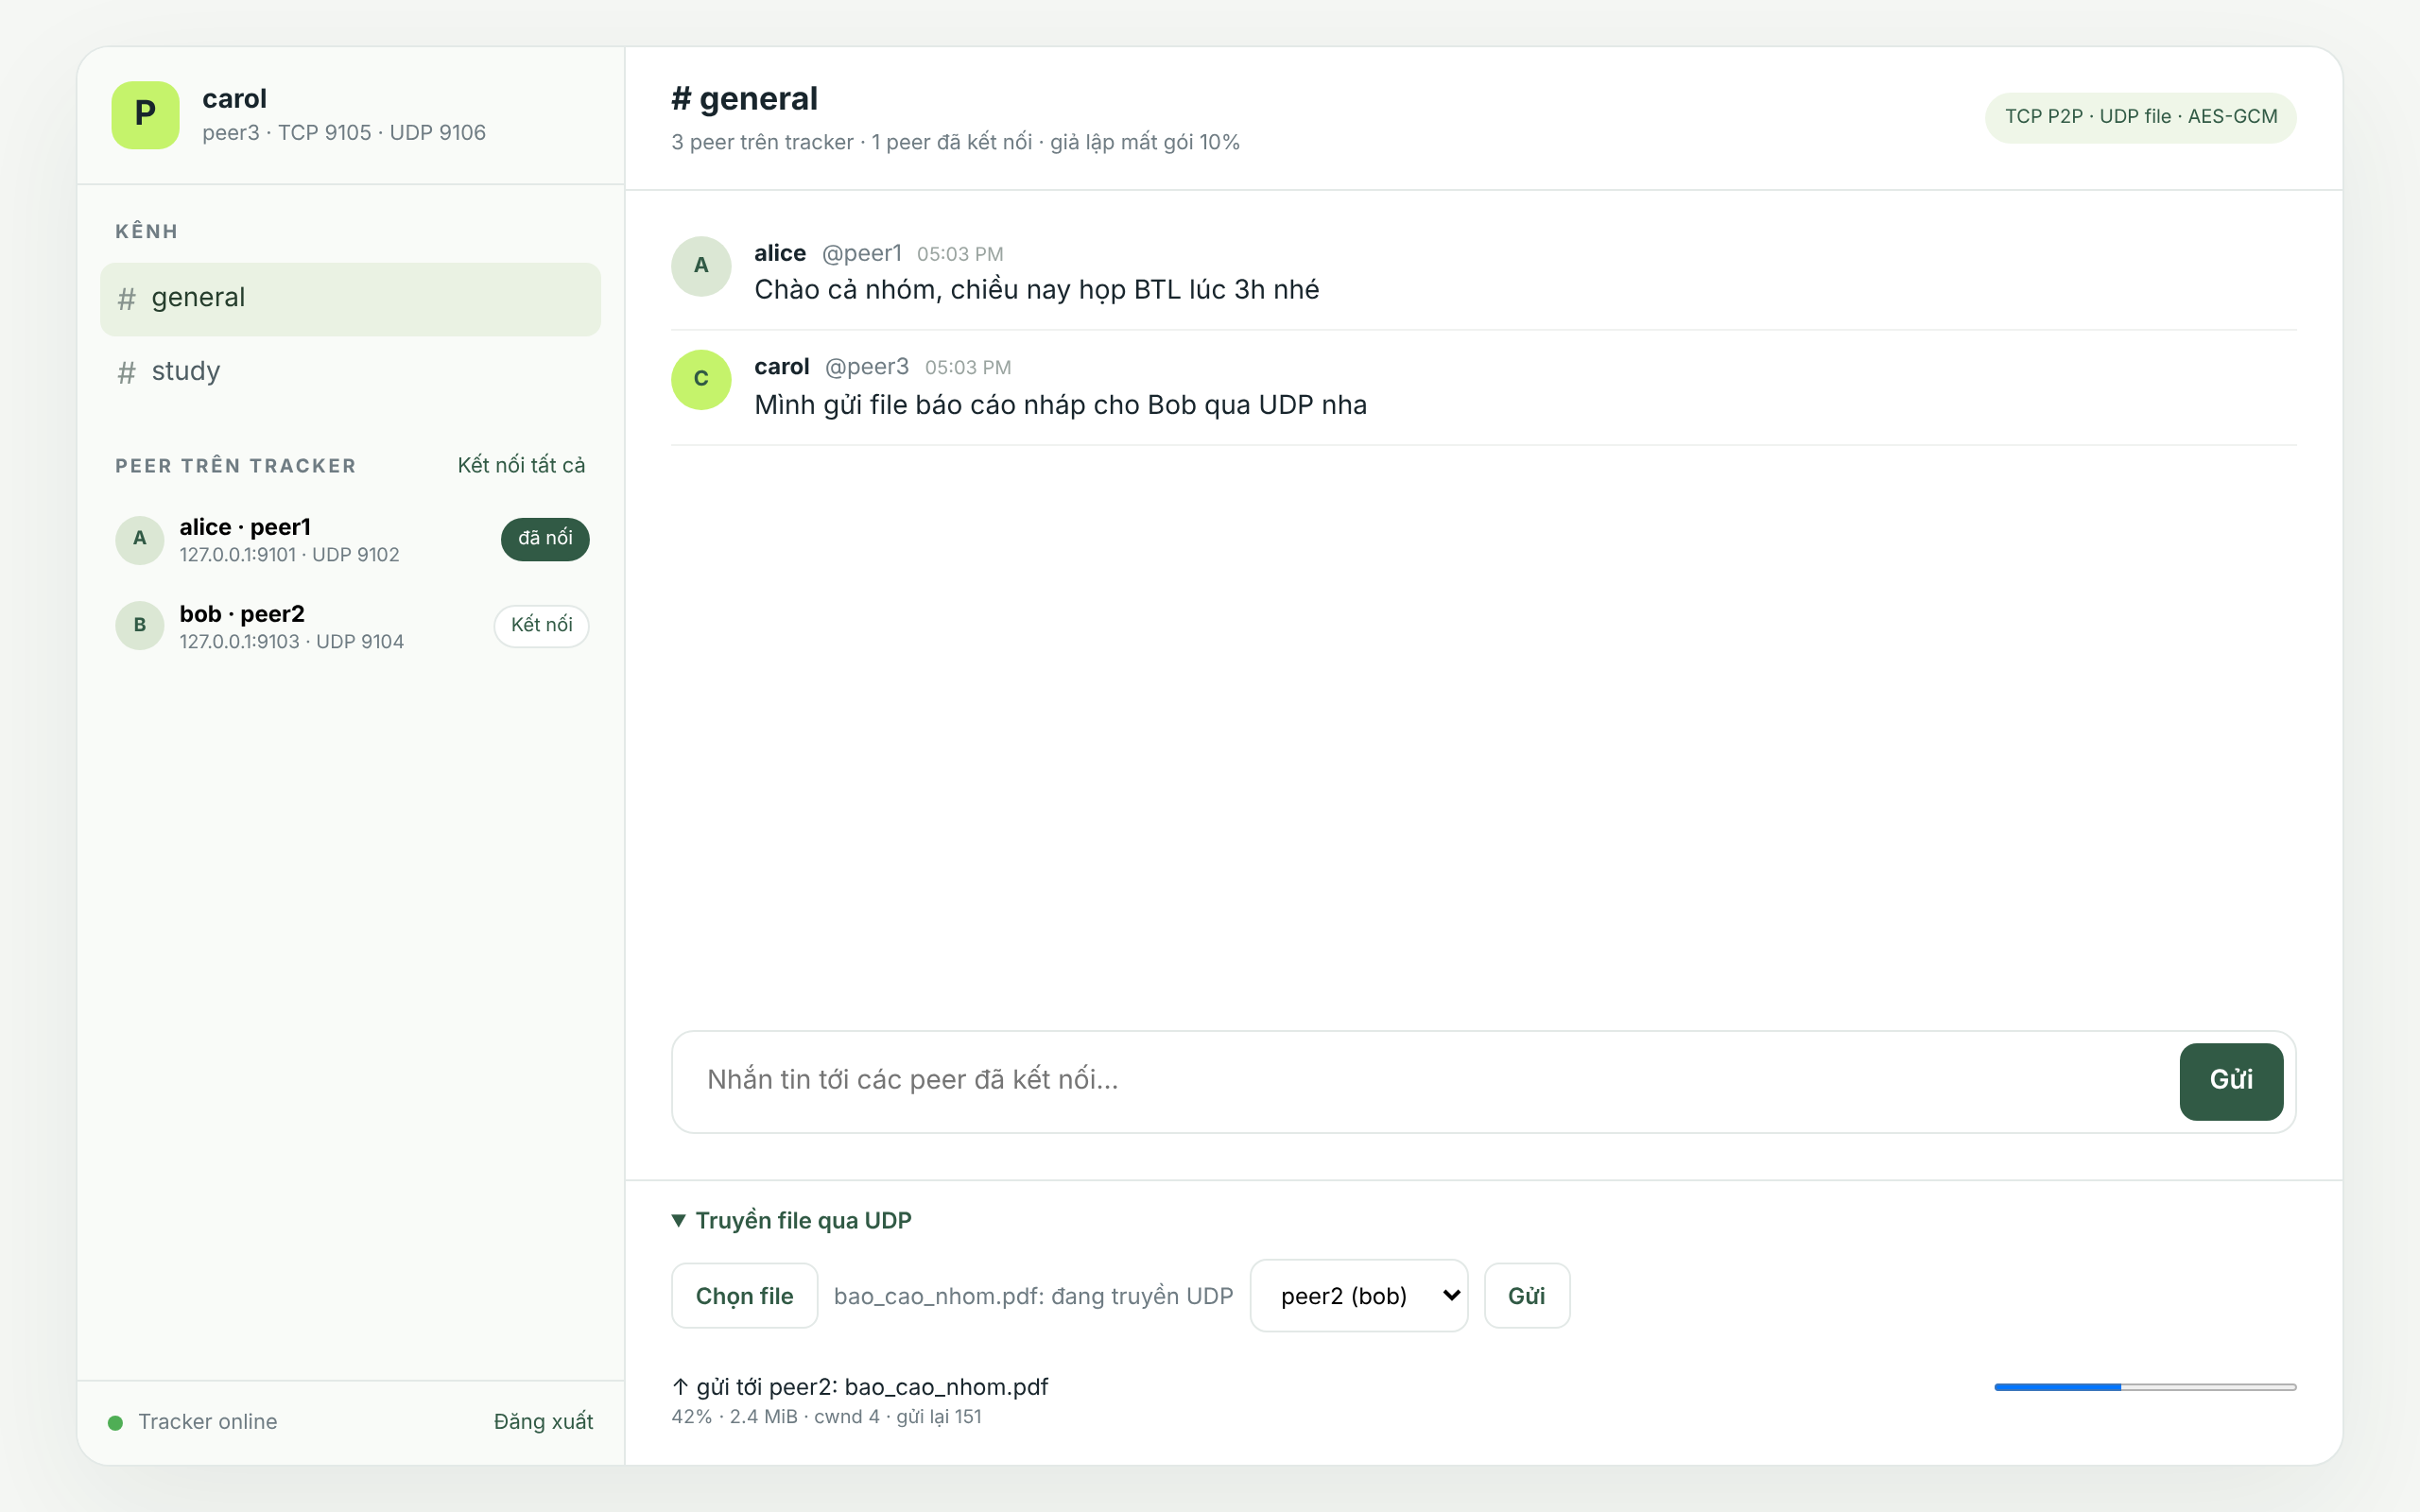
\includegraphics[width=\linewidth, trim=0 0 0 1120, clip]{figures/ui_file_progress.png}
  \caption{Sender during a transfer: 43\,\% acknowledged, \code{cwnd} = 4 after losses}\label{fig:ui-progress}
\end{subfigure}\\[4pt]
\begin{subfigure}{\textwidth}\centering
  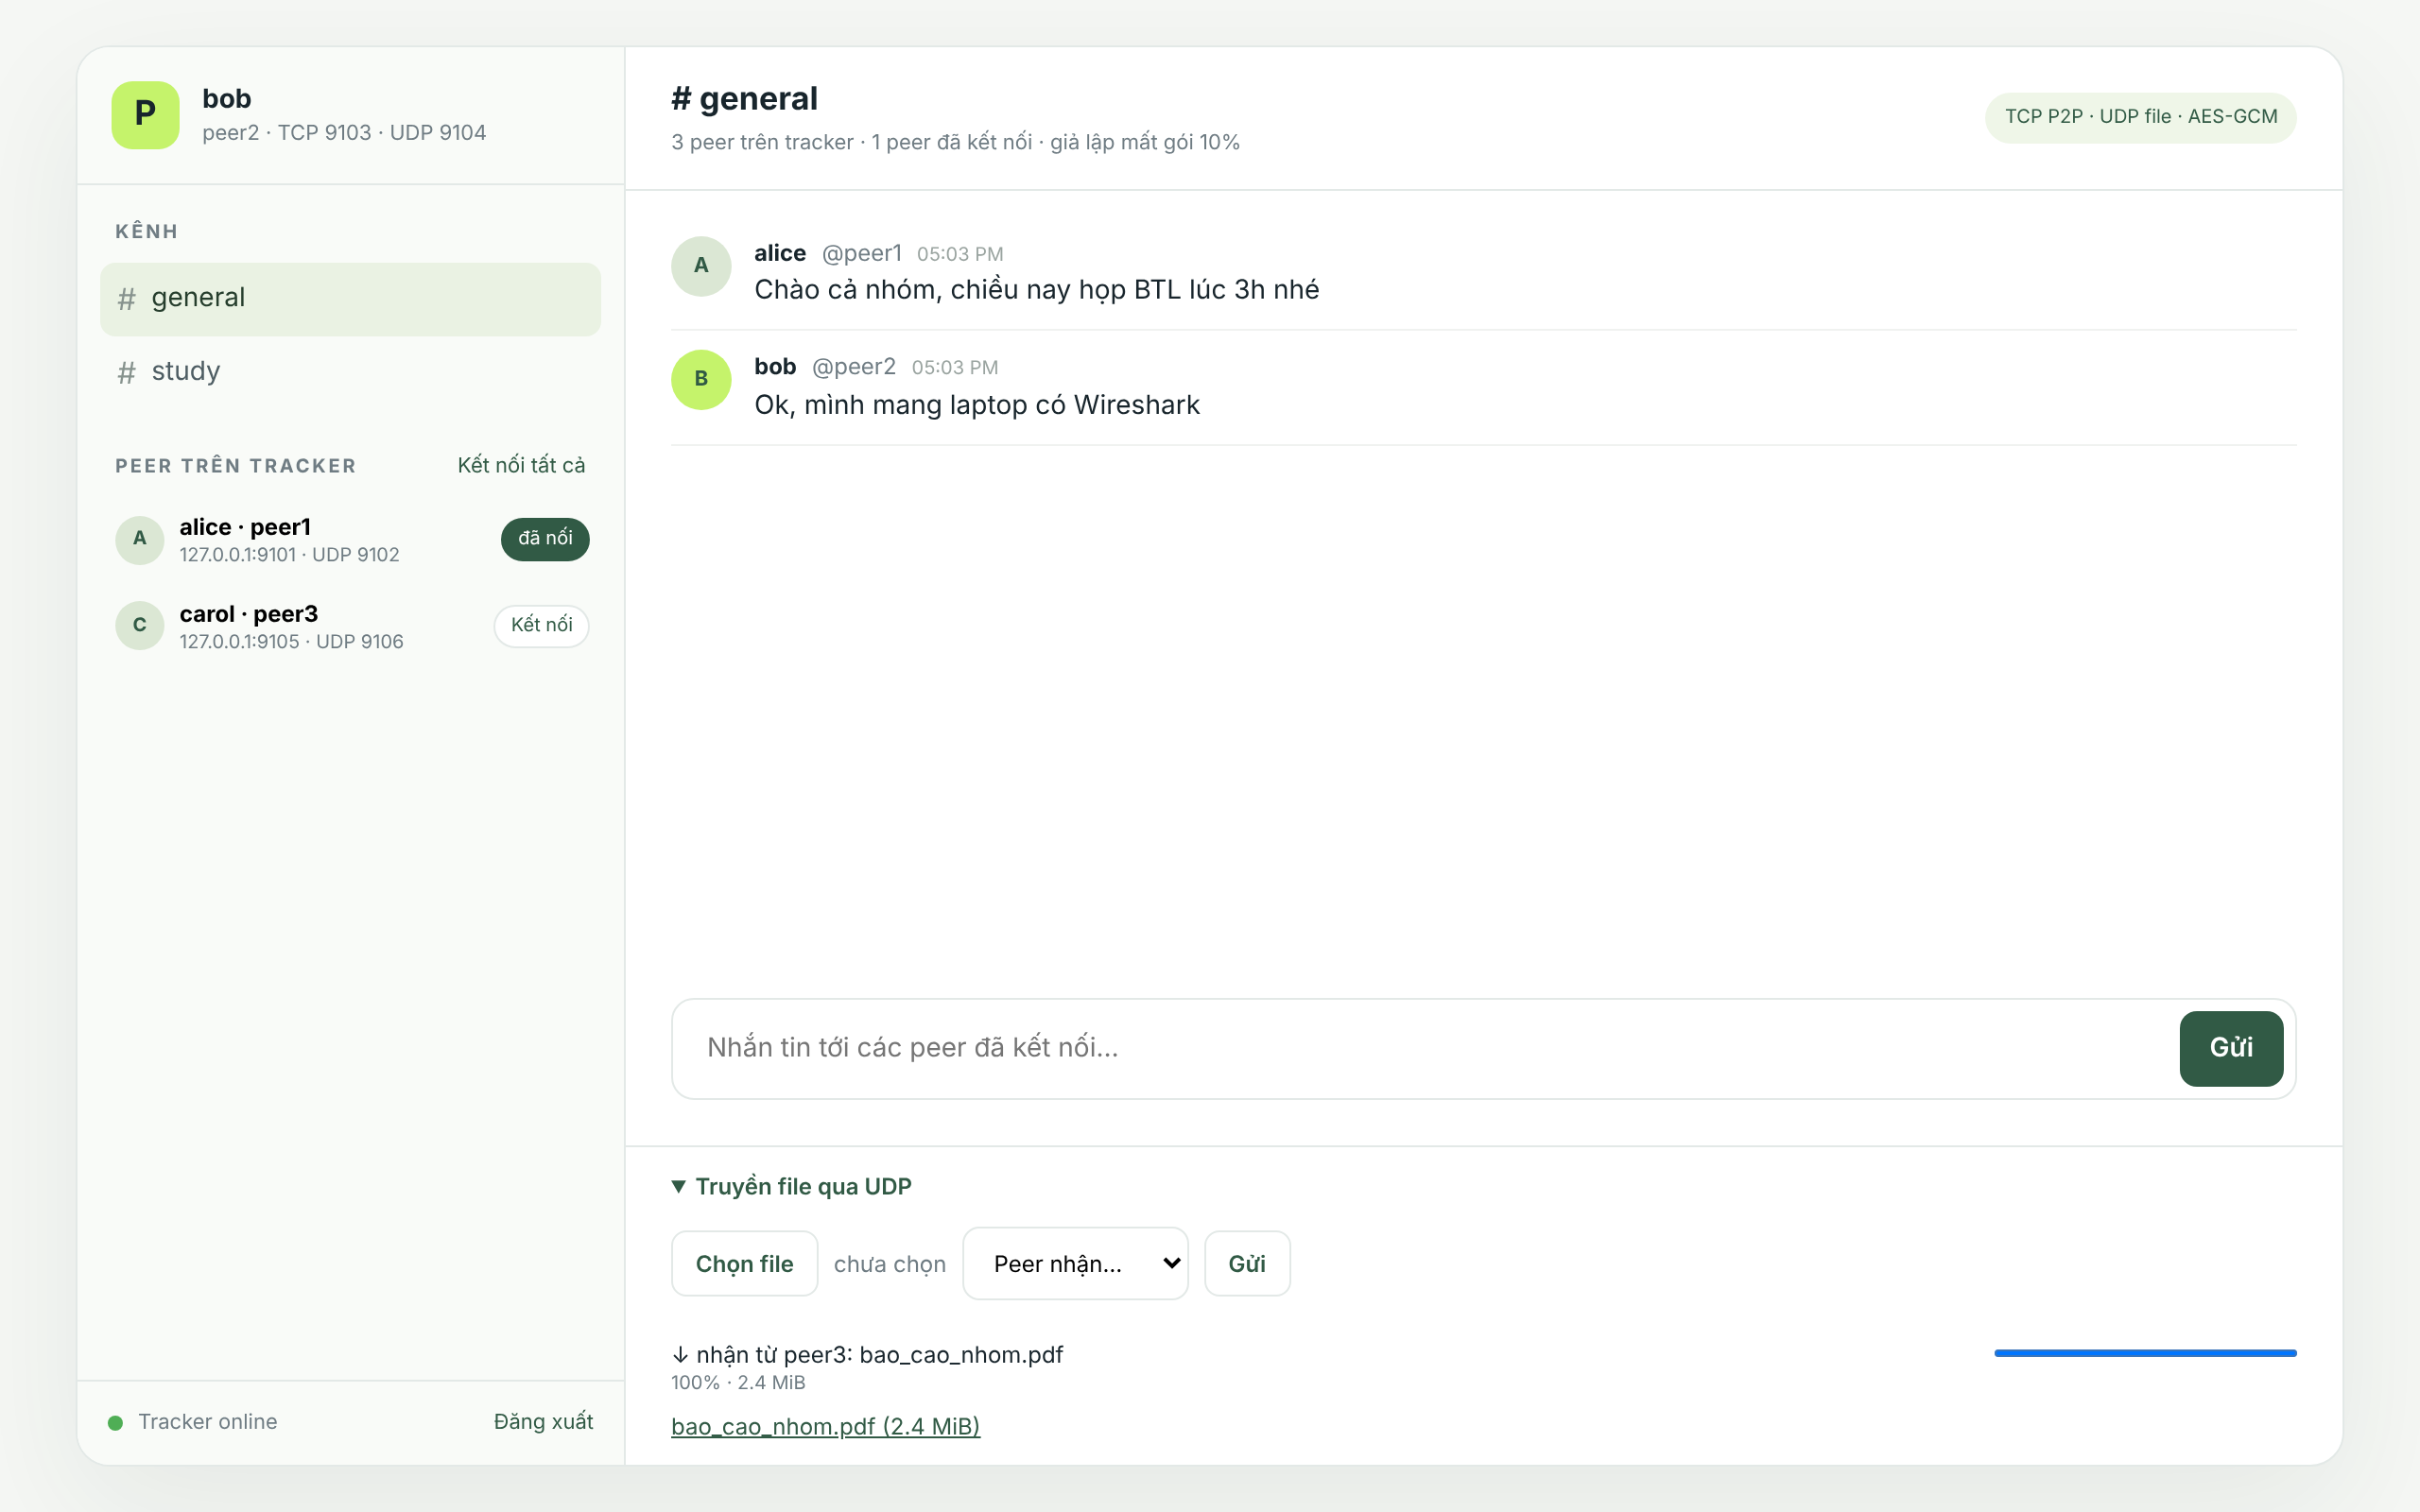
\includegraphics[width=\linewidth, trim=0 0 0 1120, clip]{figures/ui_receiver.png}
  \caption{Receiver: transfer finished, file ready to download}\label{fig:ui-receiver}
\end{subfigure}
\caption{File transfer panel (bottom of the page)}\label{fig:ui-files}
\end{figure}

The tracker serves a small status page with the peers it knows (\cref{fig:ui-tracker}); the
\emph{Seen from} column is the address the tracker observed, which helps to diagnose a wrong
\code{--peer-host} on a LAN.

\fig[fig:ui-tracker]{ui_tracker.png}{Status page of the tracker}{0.75\textwidth}
